\documentclass{standalone}
\usepackage[ascii]{inputenc}
\usepackage{tikz}

\usetikzlibrary{patterns}

\begin{document}

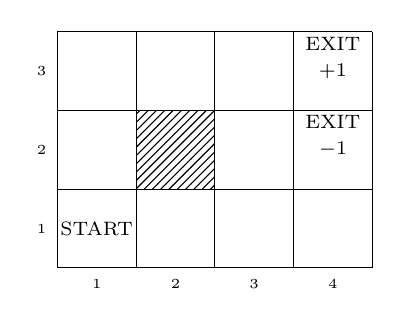
\begin{tikzpicture}
\draw (0,0) grid (4,3);
\draw [pattern=north east lines] (1,1) rectangle (2,2);
\node at (0.5,-0.2) {\tiny 1};
\node at (1.5,-0.2) {\tiny 2};
\node at (2.5,-0.2) {\tiny 3};
\node at (3.5,-0.2) {\tiny 4};
\node at (-0.2,0.5) {\tiny 1};
\node at (-0.2,1.5) {\tiny 2};
\node at (-0.2,2.5) {\tiny 3};
\node at (0.5,0.5)  {\scriptsize START};
\node at (3.5,1.85) {\scriptsize EXIT};
\node at (3.5,2.85) {\scriptsize EXIT};
\node at (3.5,1.5)  {\scriptsize $-1$};
\node at (3.5,2.5)  {\scriptsize $+1$};
\end{tikzpicture}

\end{document}
